%% ZeroCrowd-Labs — Elsevier Computers & Security manuscript (3p, two-column)
%% Compile: see paper/README-paper.md (pdfTeX driver in paper/tools/).
%% On a standard TeX Live installation: pdflatex main.tex (x3).
\documentclass[3p,twocolumn,authoryear]{elsarticle}

\usepackage{amsmath}
\usepackage{graphicx}
\usepackage{booktabs}
\usepackage{array}
\usepackage{tabularx}
\usepackage{url}
\usepackage{color}
\definecolor{passgreen}{rgb}{0.0,0.45,0.30}
\definecolor{partialamber}{rgb}{0.75,0.45,0.0}

\journal{Computers \& Security}

\begin{document}
\emergencystretch=1.5em
\renewcommand{\topfraction}{0.92}
\renewcommand{\bottomfraction}{0.85}
\renewcommand{\textfraction}{0.06}
\renewcommand{\floatpagefraction}{0.75}
\renewcommand{\dbltopfraction}{0.92}
\renewcommand{\dblfloatpagefraction}{0.75}
\setcounter{topnumber}{4}
\setcounter{dbltopnumber}{4}
\setcounter{totalnumber}{6}

\begin{frontmatter}

\title{From Owned Virtual Appliances to Scored Container Replicas:\\
Configuration Parity, End-of-Life Package Repair, and Skill-Guided
Conversion of Cybersecurity Laboratory Hosts}

\author{ZeroCrowd-Labs Project Team}
\address{ZeroCrowd-Labs open research artifact repository\\
\textit{Corresponding author to be named on submission.}}

\begin{abstract}
Cybersecurity laboratories depend on vulnerable virtual machines (VMs),
yet a full guest---its own kernel, disk, and reserved memory---is an
expensive unit to store, start, and reproduce. This paper asks whether
an owned virtual appliance can be replaced by a Docker Compose replica
that exposes the same laboratory host, and how completeness of such a
replacement should be judged. We contribute (i) a six-step,
skill-guided conversion procedure with explicit precondition and stop
conditions for importing, offline administration, end-of-life package
repair, inventory, replica construction, and parity scoring; (ii) an
eleven-row configuration-parity rubric (listening ports, unpublished
loopback services, package versions, users, sudoers, virtual hosts, web
paths, databases, cron, mail, and application URL) scored as pass,
partial, or missing, with a mandatory register of structural gaps that
may never be promoted to passes; and (iii) a validated evaluation over
eight laboratory replicas (88 rubric rows). The replicas pass 73 rows
(83.0\%; 95\% Wilson interval [73.8, 89.4]), partially satisfy 15, and
miss none, while their configured memory caps total 5,248~MB against
8,168~MB of guest RAM (35.7\% lower; caps are configuration, not measured
residency). Package versions (partial in six of eight labs) and
listening ports (four of eight) dominate the partial rows, for reasons
we trace to archive-revision drift, non-Debian guests, and nested
container topologies. In a within-case longitudinal comparison, codifying
the conversion rules raised one replica from 5 pass / 6 partial to
11 pass / 0 partial. A controlled file-lookup study (23 rule sentences,
five repetitions) confirms that the decision rules reside in the skill
documents (23/23 sentences) and are not recoverable from finished build
files (7/184 lab-file hits). We report a data-validation audit that
corrects three inconsistencies in the source record, and we delimit
every claim: no second-agent timing, no measured memory residency, and
no kernel equivalence is claimed.
\end{abstract}

\begin{keyword}
cybersecurity laboratories \sep cyber range \sep containers \sep
virtual machines \sep configuration parity \sep reproducibility \sep
end-of-life packages \sep LLM agents
\end{keyword}

\end{frontmatter}

\section{Introduction}
\label{sec:intro}

\subsection{Problem statement}

Hands-on cybersecurity education and research rely on laboratories in
which a learner or evaluator interacts with a deliberately configured
host: published services invite enumeration, loopback-only services
reward foothold thinking, and accounts, privilege rules, scheduled
jobs, and mail complete the system under study \citep{du2007,
thompson2018, yamin2020}. Community appliances distributed as virtual
machine (VM) images---VulnHub-style ``boot-to-root'' boxes are the
canonical example---package that host as a complete guest: its own
kernel, a multi-gigabyte disk, and a reserved block of RAM whether or
not the services are busy. Cyber-range research has repeatedly
identified the cost of provisioning, resetting, and scaling such
guests as a limiting factor, and container-based ranges have answered
with lighter, faster-to-deploy scenarios \citep{chouliaras2023,
nakata2021, ukwandu2020}. Containers, however, change the object being
delivered. A container shares the host kernel, replaces the guest init
system with a supervisor or a single process, and is usually rebuilt
from current packages rather than from the guest's historical ones
\citep{boettiger2015, sultan2019}. The laboratory may still \emph{answer}
on the expected port while silently ceasing to be the same host:
a database engine has been substituted, a stored application URL has
been rewritten, a loopback mail listener has vanished, or package
versions have drifted to whatever the archive serves today.

This creates a measurement problem before it creates an engineering
one. ``The page loads'' is not a fidelity criterion. What is needed is
an explicit, checkable definition of \emph{sameness} between an owned
appliance and its container replica, a conversion procedure that can
reach that definition repeatedly, and an honest account of what can
never be made the same. Those three needs---a rubric, a procedure, and
a gap discipline---motivate the present work.

A second difficulty is procedural scale. Converting one old appliance
is a long chain of preconditioned operations: importing an appliance
archive (OVA) without disturbing other guests, recovering local
administration from a powered-off disk clone without attacking the
running machine, repairing package management on an end-of-life (EOL)
distribution whose suites have left the active mirrors, inventorying
the guest without recording secrets, building a replica that keeps
loopback services unpublished, and scoring the result against the
inventory rather than against the build recipe. Each step contains
traps that \emph{look} successful locally---a newer base image that
installs cleanly, a database TCP probe that succeeds while the
application uses a different Unix socket, a supervisor that reports a
mail daemon ``stopped'' during its first minute of startup. When the
work is performed or assisted by a language-model (LM) agent, an
additional risk appears: the reasoning that avoided a trap in one
session does not automatically survive into the next conversion
\citep{yao2023}. The finished Dockerfile records the settings that
were chosen; it does not record the conditions under which a different
setting would have been a failure.

\subsection{Contributions}

This paper makes three contributions.

\textbf{C1---A skill-guided conversion procedure (Section~\ref{sec:method}).}
We formalise the conversion as six persistent procedural documents
(\emph{skills}), applied in precondition order: (1)~import onto an
existing NAT network, (2)~offline administrator recovery on a disk
clone, (3)~EOL package-archive repair under stated trust limits,
(4)~secret-redacting guest inventory, (5)~pinned replica construction,
and (6)~eleven-row parity scoring. Each skill states when it applies,
what must already be true, the commands that count, the verification
that closes the step, and the conditions under which the agent must
stop. Traps discovered during scoring are written back into the skills,
so the procedure---not a single session's transcript---is the durable
artifact, in the checklist tradition studied by \citet{haynes2009}.

\textbf{C2---A configuration-parity rubric with a non-promotable gap
register (Sections~\ref{sec:method}--\ref{sec:impl}).} Completeness is
scored on eleven rows---listening ports; unpublished loopback services;
package versions; users; sudoers; virtual hosts; web paths; databases;
cron; mail; and the application URL---each marked \emph{pass},
\emph{partial} (present with a stated substitution), or \emph{missing}
(absent, or a loopback-only service published). Three facts are kept in
an explicit gap register even when every row passes: archive or
snapshot package sources were required, the container shares the host
kernel, and a process supervisor replaces the guest init system. A
report that prints a password, hash, or flag value fails irrespective
of its row scores. The rubric operationalises, for VM-to-container
conversion, the outcome discipline that \citet{jimenez2024} argue
software-agent evaluation requires: success is a completed check, not
a plausible narrative.

\textbf{C3---A validated, multi-laboratory evaluation with an audit
trail (Section~\ref{sec:eval}).} We apply the procedure and rubric to
eight finished replicas spanning Debian~8--10, Ubuntu~14.04--18.04,
CentOS~7, a Slackware-style live system, OpenBSD~5.9, single-container
labs, a two-guest lab, and a nine-container lab (88 rubric rows). We
quantify fidelity, configured-memory reduction, the anatomy of partial
rows, and---in a single-case longitudinal study---the effect of
codifying the rules (5~pass/6~partial before codification;
11~pass/0~partial after). We complement the case evidence with a
controlled lookup study showing where the decision rules textually
reside. Crucially, every number in the paper was re-derived from the
primary artifact files by an automated validation script; three
inconsistencies in the narrative record (most materially, a ninth
replica scored in the files but described as ``not converted'' in the
project README) are corrected and handled by a sensitivity analysis
rather than silently inherited (Section~\ref{sec:eval-setup}).

\subsection{Related work}
\label{sec:related}

\paragraph{Cyber ranges and hands-on laboratories.}
\citet{yamin2020}, writing in this journal, taxonomise cyber ranges by
architecture, scenarios, functions, and tools, and \citet{ukwandu2020}
review range and testbed trends toward lighter, more composable
infrastructure. The SEED project established the value of standardised,
reproducible hands-on security exercises \citep{du2007}; Labtainers
showed that Docker containers can deliver consistent, individually
parameterised exercises on modest student hardware with automated
assessment \citep{thompson2018}; and SecGen addressed the static nature
of vulnerable VMs by generating randomised vulnerable scenarios
\citep{schreuders2017}. Container-native ranges go further:
UNIWA's autonomous platform builds complex topologies from
infrastructure-as-code on container services \citep{chouliaras2023},
while CyExec* reports near-perfect vulnerability reproducibility with
roughly half the memory and a fraction of the storage of VM scenarios
\citep{nakata2021}. That literature optimises scenario
\emph{delivery}. It does not define when a container rebuilt from a
\emph{specific owned appliance} may be said to reproduce that
appliance's listeners, accounts, package revisions, and stored
application state---the fidelity question studied here. Our replicas
are also not redistributed vulnerable images: they are local replicas
of owned appliances, built and scored under the containment rules of
Section~\ref{sec:impl}.

\paragraph{Containers versus virtual machines.}
\citet{felter2015} found containers matching or exceeding VMs on most
performance measures, \citet{bernstein2014} and \citet{merkel2014}
describe the packaging model that makes containers cheap to build and
start, and \citet{naik2016} simulates operational gains from migrating
VM deployments to Docker. \citet{sultan2019} catalogue the security
price of the shared-kernel model. Those results motivate replacing a
guest with a container and simultaneously explain why the replacement
cannot be total: kernel, init, and device behaviour are structurally
different. Our gap register is the reporting device that keeps that
difference visible after the port numbers start answering.

\paragraph{Reproducible environments and package archaeology.}
\citet{boettiger2015} frames Docker as an answer to computational
irreproducibility; \citet{nust2020} distil Dockerfile practice,
including stated base images and pinned versions; \citet{lamb2022}
treat reproducible builds as a supply-chain integrity check; and
\citet{caneill2017} document two decades of Debian history that current
mirrors no longer serve. The conversion problem adds an agent-facing
question none of those papers answers: when an EOL suite survives only
on an archive or dated snapshot, under exactly what conditions may an
agent disable validity-window checking, add \texttt{trusted=yes}, or
pin a snapshot---and how must that repair be reported so it is not
mistaken for fidelity? Section~\ref{sec:method} states those rules and
Section~\ref{sec:eval} scores their consequences.

\paragraph{Infrastructure-as-code verification.}
\citet{guerriero2019} report that practitioners lack practical tests
for infrastructure code; \citet{hummer2013} test configuration
automations for idempotence; and \citet{shambaugh2016} verify Puppet
configuration determinacy with a solver. The parity rubric is a weaker,
empirical relative: it compares a running replica against a redacted
guest inventory, row by row, from live evidence (\texttt{ss},
\texttt{dpkg-query}/\texttt{rpm -q}, HTTP status, \texttt{visudo -c}),
and it fails closed---a non-running replica scores its runtime rows
missing rather than inheriting the Dockerfile's intentions.

\paragraph{Agents, checklists, and outcome-based scoring.}
\citet{yao2023} interleave reasoning and tool use, but the plan is
generated inside the episode; a skill inverts that arrangement by
making the procedure persistent and prior to the episode.
\citet{haynes2009} show---in a clinical setting whose effect sizes we
do \emph{not} transfer---that checklists change work of this shape by
making required actions and pause points explicit. \citet{jimenez2024}
score LM software agents by completed issue resolution (their strongest
evaluated model resolved 1.96\% of 2,294 real issues); we adopt the
outcome discipline, not the benchmark: our check is parity, and a
shared kernel may not be scored as reproduced. No prior work we are
aware of states a VM-to-container parity rubric, the EOL-apt trust
rules, or the supervisor/mail scoring traps for this conversion task.
Table~\ref{tab:related} positions the contribution against the closest
literature.

\begin{table*}[tbp]
\caption{Positioning against related work. ``---'' means the work does
not address the dimension. This paper is the only row that combines a
VM-specific parity rubric, EOL-archive trust rules, and a
non-promotable kernel/init gap register.}
\label{tab:related}
\centering\footnotesize
\begin{tabularx}{\textwidth}{>{\raggedright\arraybackslash}X>{\centering\arraybackslash}X>{\centering\arraybackslash}X>{\centering\arraybackslash}X>{\centering\arraybackslash}X>{\centering\arraybackslash}X}
\toprule
Work & Container labs & Fidelity rubric & EOL rules & Gap register & Procedure\\
\midrule
Yamin et al. (2020); Ukwandu et al. (2020) & Survey & --- & --- & --- & ---\\
SEED (Du et al., 2007); Labtainers (Thompson \& Irvine, 2018) & Yes & --- & --- & --- & ---\\
SecGen (Schreuders et al., 2017) & VM generation & --- & --- & --- & ---\\
UNIWA CR (Chouliaras et al., 2023); CyExec* (Nakata \& Otsuka, 2021) & Yes & Scenario-level & --- & Kernel limits noted & ---\\
Felter et al. (2015); Naik (2016); Sultan et al. (2019) & Performance/security & --- & --- & Kernel analysed & ---\\
Boettiger (2015); N\"ust et al. (2020); Lamb \& Zacchiroli (2022) & Packaging & Version pinning & Historical suites & --- & ---\\
Guerriero et al. (2019); Hummer et al. (2013); Shambaugh et al. (2016) & IaC testing & Config. checks & --- & --- & ---\\
ReAct (Yao et al., 2023); SWE-bench (Jimenez et al., 2024) & --- & Task success & --- & --- & In-episode\\
\textbf{This paper} & \textbf{Replica of owned VM} & \textbf{11-row parity} & \textbf{Archive/snapshot rules} & \textbf{Kernel, init, archive} & \textbf{Persistent skills}\\
\bottomrule
\end{tabularx}
\end{table*}

\subsection{Scope, ethics, and paper organisation}

The study covers owned appliances converted and run locally for
education and evaluation. It contributes no attack procedure: the
parity report deliberately contains no exploit steps, credentials,
hashes, or flag values, and inventorying stops at version recording
where a check would require attacking a service. Student-facing
variants rebuild the same topologies on a current Debian~12 base with
\texttt{PermitRootLogin no} and learner-chosen passwords
(Section~\ref{sec:impl}). Section~\ref{sec:method} defines the method
(research questions, procedure, rubric, deployment model, and evidence
discipline). Section~\ref{sec:impl} describes the implementation
mechanics. Section~\ref{sec:eval} presents the experimental design and
results. Section~\ref{sec:discussion} discusses interpretation,
security implications, validity threats, and limitations.
Section~\ref{sec:conclusion} concludes.

\section{Methodology}
\label{sec:method}

\subsection{Research questions and design overview}

The study is an artifact-centred case series with one embedded
longitudinal case and one controlled text-lookup study. It follows
case-study and empirical-reporting discipline for software and systems
artifacts \citep{kitchenham2002, runeson2009, wohlin2012}: research
questions are fixed first, evidence sources are named before results,
and every quantitative claim is traceable to a primary file.

\begin{itemize}
\item \textbf{RQ1 (Fidelity).} How completely do skill-guided container
replicas reproduce their owned guest appliances under an eleven-row
configuration-parity rubric, and where do partial rows concentrate?
\item \textbf{RQ2 (Resource configuration).} How do configured replica
memory caps compare with guest RAM allocations, and is any fidelity
difference associated with the size of the configured saving?
\item \textbf{RQ3 (Rule codification).} Within the one lab scored before
and after the rules were codified (Raven), which rows changed, and what
did the fixes consist of?
\item \textbf{RQ4 (Rule residence).} Are the decision rules recoverable
from the finished build files alone, or do they reside in the skill
documents an agent is instructed to read?
\end{itemize}

RQ1 and RQ2 are answered descriptively over the eight-lab corpus
(Section~\ref{sec:eval-results}). No null-hypothesis test is offered
for them: labs are heterogeneous cases, rubric rows within a lab are
not independent trials, and $n=8$ cannot support population inference.
Two exploratory Spearman correlations are reported \emph{as
exploratory}, with their sample size attached. RQ3 is a single-case
before/after comparison and is interpreted as such---it demonstrates
that the codified rules address the observed failure modes, not that
codification caused a measured agent speedup. RQ4 is answered by exact
string lookup, a measurement of text residence; we are explicit that
file-read milliseconds are not language-model latency and that no
second agent was timed.

\subsection{The six-skill conversion procedure}

Figure~\ref{fig:method} shows the pipeline and Figure~\ref{fig:deploy}
the resulting deployment architecture. Table~\ref{tab:skills} states
each skill's contract. The ordering is by precondition, not by
convenience: inventory before build (the build consumes inventory
facts, not guesses), archive repair before inventory where the guest
must be booted to be inventoried, and scoring last and independently
of the build recipe.

\begin{figure*}[tbp]
\centering
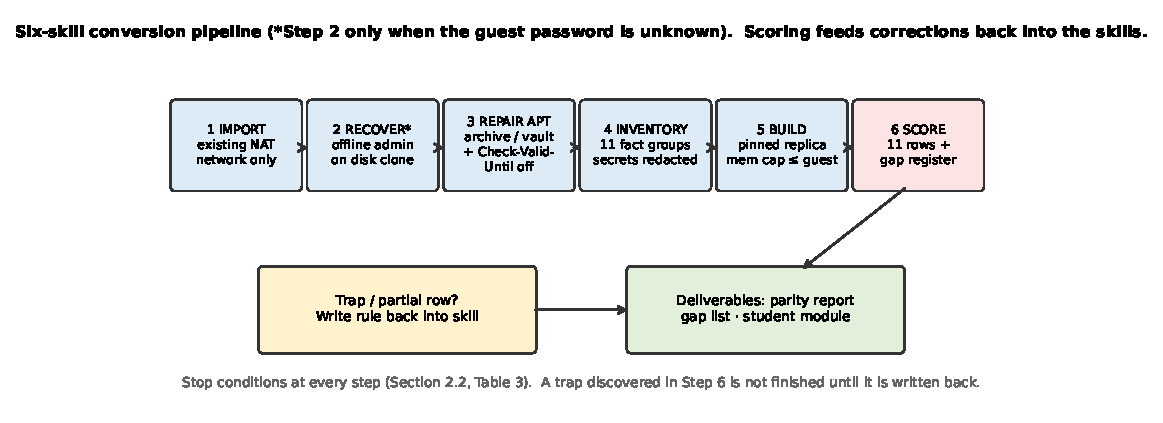
\includegraphics[width=\textwidth]{figures/fig02_methodology.pdf}
\caption{Six-skill conversion pipeline. Step~2 is conditional (unknown
guest password). Scoring (Step~6) is performed from live evidence, and
any trap or partial row it exposes is written back into the responsible
skill before the replica is treated as finished.}
\label{fig:method}
\end{figure*}

\begin{figure*}[tbp]
\centering
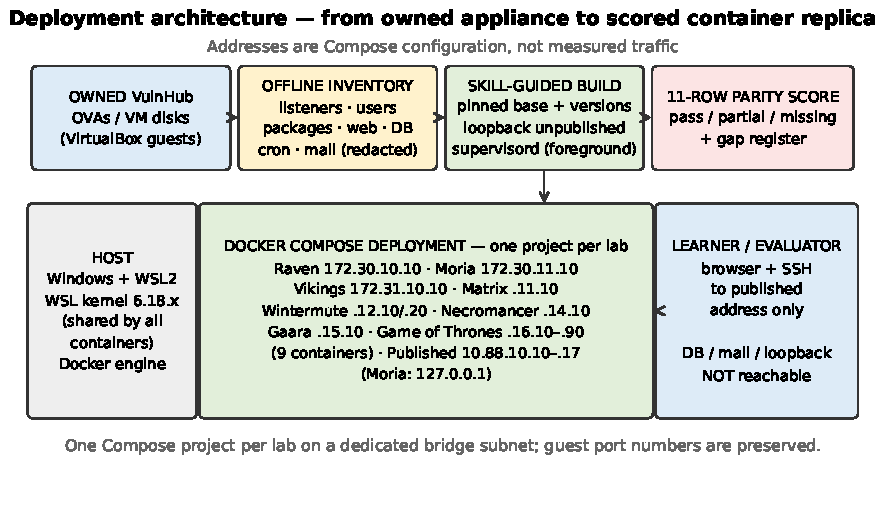
\includegraphics[width=\textwidth]{figures/fig01_deployment.pdf}
\caption{Deployment architecture. One Compose project per lab on a
dedicated bridge subnet; publication only on a dedicated local address
range (10.88.10.10--.17; Moria is the loopback-published exception).
Container addresses (172.30/172.31.*) and published addresses are
different layers of the same deployment and are both configuration, not
measured traffic.}
\label{fig:deploy}
\end{figure*}

\textbf{Step 1---Import (\texttt{importing-ova-nat\-network}).} Register
exactly one appliance in VirtualBox; attach only that VM's enabled
adapters to a pre-existing NAT network; record the VM list before and
after. \emph{Stop} if the NAT network is absent, the name collides, or
any other VM changed. This containment rule is what makes a series of
conversions composable on one host.

\textbf{Step 2---Offline recovery
(\texttt{recovering-linux-admin\-offline}; conditional).} Only when the
guest password is unknown and the machine is powered off: clone the
disk (RAW), mount the clone (handling LVM via device-mapper nodes where
necessary), add a local administrator (uid $\geq$ 1000, \texttt{sudo} on
Debian/Ubuntu, \texttt{wheel} elsewhere) and set passwords inside the
mount, verify by login (serial console where available), and convert
back. The operator password is chosen at runtime and is never written
to a skill, inventory, or report. \emph{Stop} rather than escalating to
an online attack; an encrypted (LUKS) root without a passphrase is a
terminal stop.

\textbf{Step 3---EOL package repair
(\texttt{repairing-eol-apt\-archives}).} When \texttt{apt-get update}
fails because the suite left the active mirrors: keep suite and
component names, rewrite hosts to \texttt{archive.debian.org} /
\texttt{old-releases.ubuntu.com} (CentOS guests use the vault mirror
instead), disable the validity window
(\texttt{Acquire::Check-Valid-Until "false"}), and add
\texttt{trusted=yes} \emph{only} to archived lines that still fail with
\texttt{EXPKEYSIG}, expired signature, or \texttt{NO\_PUBKEY}. If the
old-releases host 404s while the active archive still serves the suite,
move the lines back---trust is never extended to a current mirror.
Verification is \texttt{apt-get update} and a simulated install
(\texttt{apt-get install -s bash}) both exiting~0. The repair is legal
and remains a registered gap (Section~\ref{sec:rubric}).

\textbf{Step 4---Inventory (\texttt{inventorying-linux\-vm}).} Record,
from the running guest where it can be booted and otherwise from unit
files and configuration (the provenance is itself recorded): listeners
with bind address and loopback status; human users with uid, home, and
shell; sudoers (validated with \texttt{visudo -c}); service package
version strings; virtual hosts, document roots, and web paths; the
application database name, user, host, and socket; cron (root crontab,
\texttt{cron.d}, user crontabs); and mail listeners. Passwords, hashes,
private keys, and flag values are replaced by a redaction token at
capture time.

\textbf{Step 5---Build (\texttt{building-docker-vm\-replica}).} One
Compose project per lab; base image from the guest's distribution
codename where the guest system can be a Linux container base;
\emph{pin the inventoried package revisions} (dated snapshot where the
archive no longer carries them) and do not call the package row a pass
until \texttt{dpkg-query -W} (or \texttt{rpm -q}) matches the inventory
strings; install the inventoried database engine, not a substitute
(MariaDB for MySQL is a partial until removed); publish exactly the
guest's non-loopback port numbers, on the dedicated address where one
is requested, leaving loopback services unpublished and never
renumbering guest ports to dodge a busy local port; map the guest
hostname to the published address instead of rewriting the stored
application URL; initialise the application database once, reading its
password from the configuration file as text and pointing the runtime
at the socket the server actually creates; supervise long-running
processes \emph{in the foreground} (canonically
\texttt{sendmail -bD}, not the forking \texttt{-bd}); and cap memory at
or below the guest RAM allocation. Where the guest cannot be the base
(OpenBSD, Slackware package format, a guest that itself ran a Docker
engine), the substitution is chosen deliberately and scored partial
where the rubric requires it.

\textbf{Step 6---Score (\texttt{evaluating-docker-vm\-parity}).} Score
the eleven rows from the inventory and from live commands against the
running container---never from the Dockerfile alone. A non-running
replica scores runtime rows missing. Mail is scored from listening
sockets (\texttt{ss}) after the daemon's startup delay (about a minute
for Sendmail~8.14), not from supervisor status in the first seconds.
Archive apt alone does not make matching version strings partial.
Publishing a loopback-only service is a missing row, not a convenience.
The report must contain the gap register and no secrets, hashes, flags,
or exploit steps. A seventh skill, \texttt{designing-lab\-scenarios},
consumes inventories and topologies to draft \emph{new} laboratory
briefs (hosts, published vs.\ loopback services, roles; no attack path
or credentials) and is used in teaching, not in conversion scoring.

\begin{table*}[tbp]
\caption{Skill contracts: precondition, stop condition, and closing
verification. The seventh (scenario-design) skill is not part of the
conversion chain and is therefore listed separately in the text.}
\label{tab:skills}
\centering\footnotesize
\begin{tabularx}{\textwidth}{clXX}
\toprule
Step & Skill & Stop condition (extract) & Verification that closes the step\\
\midrule
1 & importing-ova-nat-network & NAT network missing; name collision; another VM changed & VM list before/after differs only by the new guest\\
2 & recovering-linux-admin-offline & Password known; next step would be an online attack; encrypted root, no passphrase & Administrator login verified on the clone\\
3 & repairing-eol-apt-archives & \texttt{apt-get update} already exits 0; mirror still current; rewritten URL still 404s & \texttt{apt-get update} and simulated install exit 0\\
4 & inventorying-linux-vm & A secret, hash, or flag value would be recorded & Eleven fact groups recorded, secrets redacted, provenance stated\\
5 & building-docker-vm-replica & Database host non-local (single-container pattern); loopback service would be published & Image present; container running; \texttt{docker inspect} confirms cap, address, bindings\\
6 & evaluating-docker-vm-parity & Inventory missing; replica state unknown; check would require attacking a service & 11 rows scored pass/partial/missing; gap register completed\\
\bottomrule
\end{tabularx}
\end{table*}

\subsection{The parity rubric and the gap register}
\label{sec:rubric}

Table~\ref{tab:rubric} defines the eleven rows. Three design choices
deserve emphasis. First, the unit is the \emph{row}, scored strictly:
a package row passes only on string equality with the inventory
(e.g., Apache \texttt{2.4.10-10+deb8u12} is not ``close enough'' to
\texttt{2.4.25}); where several packages define a lab, the row is
partial if the defining strings differ, even if some match. Second,
\emph{partial} is a positive reporting category, not a softened fail:
it asserts the function exists with a named substitution, so readers
can see exactly what was traded. Third, \emph{missing} includes the
security-relevant inversion---publishing a service the guest kept on
loopback---because a replica that exposes a database the original kept
private is not merely incomplete, it teaches the wrong topology.

\begin{table}[tbp]
\caption{Parity rubric. Pass requires both configuration equality and
the practical result (listener present, URL answering HTTP~200, rule
parsing).}
\label{tab:rubric}
\centering\footnotesize
\begin{tabularx}{\columnwidth}{lX}
\toprule
Row & Pass criterion (summary)\\
\midrule
Listening ports & Same port numbers/process roles listening; live evidence preferred\\
Loopback unpublished & Every guest loopback listener absent from host publication\\
Package versions & Inventoried version strings equal (\texttt{dpkg-query}/\texttt{rpm -q})\\
Users & Same names, uids, homes, shells (added operator disclosed)\\
Sudoers & Same rules; \texttt{visudo -c} parses\\
Virtual hosts & Same vhost set, names, document roots\\
Web paths & Same paths present; expected HTTP status\\
Databases & Same engine and application schema (none/none passes)\\
Cron & Same crontabs and \texttt{cron.d} entries\\
Mail & Same mail package/listeners (none/none passes)\\
Application URL & Stored URL unchanged and answering\\
\bottomrule
\end{tabularx}
\end{table}

Independently of the rows, every report carries a \textbf{gap
register}: (i)~version substitutions (empty when the package row
passes); (ii)~archive/snapshot/vault package sources, where used;
(iii)~second kernel---always ``no'': the container uses the host (WSL2)
kernel, never the guest kernel; and (iv)~init substitution
(supervisord or a shell entrypoint in place of systemd/sysv/OpenBSD
\texttt{rc}), plus deployment deltas (unrecreated NICs, collapsed guest
networks, unloaded packet filters, and the configured-not-measured
memory cap). The register is the paper's central honesty device: it
makes the structurally unreproducible parts of a container conversion
impossible to launder into a pass.

\subsection{Deployment and dataset model}

Each lab is an independent Compose project with a dedicated bridge
subnet and static container addresses; learners and evaluators reach
only the published address (Figure~\ref{fig:deploy}). The dataset for
RQ1--RQ2 is the set of primary artifact files per lab:
\texttt{vm-inventory.md} (guest facts and provenance),
\texttt{replica-parity.md} (row scores, substitutions, gap register),
\texttt{docker-compose.yml}/\texttt{replica/compose.yaml} (caps,
addresses, bindings), the Dockerfile(s) (base image and pins), and,
where produced, \texttt{experiment.md} (lookup study). The
student-facing \texttt{Educational-Module.md} files are derived
teaching artifacts and are evidence only for the teaching discussion.
Section~\ref{sec:eval-setup} gives the dataset table and the audit
that validated it.

\subsection{Evidence discipline}

Three rules govern all reporting. (1)~\emph{Configuration is not
measurement}: memory figures are Compose \texttt{mem\_limit} values and
VirtualBox allocations, not resident-set measurements; addresses are
Compose configuration, not traffic captures. (2)~\emph{Provenance is
data}: inventories collected from a running guest over a serial console
are stronger evidence than inventories reconstructed from unit files of
a guest that could not be booted, and tables carry that grade.
(3)~\emph{Absence is reported}: where the record is silent (a version
string not captured in an early round, a guest never booted), the cell
stays empty and the text says so, rather than being reconstructed.


\section{Implementation---Mechanics}
\label{sec:impl}

This section describes how the method is realised in the repository:
the per-lab artifact layout, the build mechanics that make row passes
achievable, the containment and teaching surfaces, and the failure
traps that the skills now encode. It is deliberately mechanical: a
reader should be able to repeat a conversion from this section and the
skills without access to any conversion session.

\subsection{Artifact layout}

Every lab occupies \texttt{labs/<name>/} containing the Compose entry
point (\texttt{docker-compose.yml}, in most labs an \texttt{include} of
\texttt{replica/compose.yaml}), the build context (\texttt{replica/}
with Dockerfile, entrypoint, supervisor configuration, and service
configuration), \texttt{vm-inventory.md}, \texttt{replica-parity.md},
\texttt{Educational-Module.md}, and the helper scripts produced while
working the lab (disk mapping, mounting, download, and scoring
scripts). Shared skills live in \texttt{skills/}; student-copied site
files and images live in each lab's \texttt{resources/} and in the
top-level \texttt{resources/}. Disk images, appliance archives,
password files, and shadow extracts are intentionally not in the
repository: the parity system must be auditable without the secrets it
is forbidden to print. Keeping the inventory, the build, and the score
as three separate files is what makes the without-skills condition of
RQ4 well-defined---the build files are exactly what a later agent
inherits if the skills are withheld.

\subsection{Base images, pinning, and EOL repair in practice}

Replica bases follow the guest where a Linux container base exists:
\texttt{debian:jessie} (Raven), \texttt{centos:7.3.1611} (Moria),
\texttt{ubuntu:18.04} (Vikings), \texttt{debian:10} (Gaara),
\texttt{debian:9} (Game of Thrones), \texttt{ubuntu:16.04} and
\texttt{debian:stretch} (Wintermute's two containers),
\texttt{ubuntu:14.04} (MrRobot, sensitivity corpus), and
\texttt{python:2.7.14} for Matrix, whose guest is a Slackware-style
Porteus live system whose one reproducible anchor is the interpreter
version (2.7.14) rather than a distribution. Necromancer's OpenBSD~5.9
guest cannot be a base on a Linux engine, so its replica is Debian~11
with nginx standing in for OpenBSD \texttt{httpd}; both substitutions
sit in the gap register and the affected rows score partial.

Pinning is literal. Raven's Dockerfile, for example, writes six dated
snapshot pairs plus the archive lines for Jessie, sets
\texttt{Check-Valid-Until "false"} and \texttt{trusted=yes} on those
archived lines only, and pins the inventoried revisions
(Apache \texttt{2.4.10-10+deb8u12}, PHP \texttt{5.6.36+dfsg-0+deb8u1},
MySQL \texttt{5.5.60-0+deb8u1}, OpenSSH \texttt{1:6.7p1-5+deb8u4},
Sendmail \texttt{8.14.4-8+deb8u2}, cron, sudo) at priority~1001 before
installing. Moria reaches the same string equality through the CentOS
vault: its image is \texttt{centos:7.3.1611} and \texttt{rpm -q}
returns the guest strings (httpd \texttt{2.4.6-45.el7.centos},
PHP \texttt{5.4.16-42.el7}, OpenSSH \texttt{6.6.1p1-33.el7\_3}, postfix,
vsftpd, chrony). Those two labs are the corpus's only package-row
passes, and they demonstrate the rubric's asymmetry: archive use alone
does not make a row partial, but the archive's \emph{newer} security
revision does. Five labs are partial precisely because the archive now
serves a higher revision than the guest carried (e.g., Gaara's Apache
\texttt{2.4.59-1\textasciitilde deb10u1} for \texttt{2.4.38-3+deb10u4}),
which is a reproducibility fact about EOL ecosystems, not a build
error that more effort at the same mirror could remove. Where the
revision no longer exists on the archive, the build must name the
snapshot timestamp that still carries it---the mechanism Raven's six
snapshot lines encode.

Two build subtleties recur. Jessie-era apt can ignore
\texttt{trusted=yes} and fail signature validation through the
\texttt{gpgv} shim; the skill's remedy (a \texttt{Dir::Bin::gpg} stub
emitting \texttt{GOODSIG}/\texttt{VALIDSIG} for the archived suite
only, or \texttt{--force-yes} where that apt requires it) is scoped to
the archived lines for exactly the trust reason stated in Step~3.
And database initialisation is one-shot: a volume initialised by one
engine may not be mounted into the other---in Raven, the MySQL~5.5
volume had to be created fresh after the MariaDB substitution was
removed, a rule the build skill now states explicitly.

\subsection{Supervision, sockets, and the mail trap}

Containers have no guest init, so entrypoints supervise the inventoried
daemons in the foreground under supervisord (or, for Moria and single-
process Game-of-Thrones containers, a shell entrypoint or the daemon's
own foreground mode). Three mechanical rules in the skills come from
observed mis-scores. First, \emph{foreground means foreground}:
\texttt{sendmail -bd} forks and exits, so the supervisor marks the
program stopped while a child may still listen; \texttt{sendmail -bD}
stays in the foreground and is the supervised form. Second, \emph{score
the socket, not the supervisor}: Sendmail~8.14 sleeps for roughly a
minute after its startup DNS/syslog attempts, so ports~25/587 are
scored from \texttt{ss} after that window; shortening resolver timeouts
and providing \texttt{/dev/log} did not remove the sleep, which is why
the rule is a wait, not a configuration change. Third, \emph{the
application's socket is the server's socket}: PHP's MySQL socket path
is configured (\texttt{mysql-socket.ini} in both the Apache and CLI
PHP configurations in Raven) to the socket the installed server
creates (\texttt{/var/run/mysqld/mysqld.sock}); a successful TCP probe
on 3306 does not evidence this, and an earlier build generation that
trusted it scored the database row on the wrong signal. Equivalent
small mechanics appear across the corpus: rpcbind plus foreground
\texttt{rpc.statd} restores Raven's NFS listener row; Moria's chrony
needs \texttt{CAP\_SYS\_TIME} in the container
(\texttt{cap\_add: SYS\_TIME}) and its vsftpd is run IPv4-only with
\texttt{background=NO}; Game of Thrones runs nine single-process
containers (SSH, Apache, nginx$\times$2, BIND, Dovecot, MariaDB,
PostgreSQL, pure-ftpd) on one bridge because the guest itself was a
Docker host---reproducing its topology, not its engine.

\subsection{Networking and publication mechanics}

Publication is the security-critical mechanic. Compose binds only the
inventoried non-loopback port numbers, and binds them to a dedicated
local address (10.88.10.10--.17 in the primary corpus) rather than to
all interfaces or to a contended 127.0.0.1. That choice preserves the
guest's port numbers---a rubric requirement---without colliding with
other replicas' loopback publications, and it keeps the stored
application URL honest: Raven serves
\texttt{http://raven.local/wordpress/} with the hostname mapped to the
published address (\texttt{extra\_hosts} / hosts entry) instead of
rewriting WordPress's stored URL to a raw address, which an earlier
generation did and which the rubric counts partial. Loopback services
(MySQL on 3306, Sendmail on 25/587, Redis on 6379, SNMP on 161/udp,
Tomcat's shutdown port, Necromancer's entire HTTP/SNMP/Python set,
Vikings' RPyC server on 18812) are present inside the container where
the guest had them and absent from the Compose publication list;
Docker's embedded resolver (127.0.0.11) is likewise never published.
Moria is the documented exception, publishing 21/22/80 on 127.0.0.1,
and Necromancer is the limiting case: only SSH is published and its
application URL answers only inside the container, which the rubric
scores as a pass because that \emph{is} the guest topology. Guest
networks that cannot be recreated (Wintermute's two host-only
networks, Game of Thrones' eight isolated container networks) collapse
to the lab bridge and are recorded as gaps.

\subsection{Containment, secrets, and the teaching surface}

The conversion workflow is contained at each step: appliances attach
only to an existing NAT network; offline administration edits a
\emph{clone}, never the registered disk, and never a running machine;
inventory redacts at capture; parity reports fail if they contain
secrets. The teaching surface is deliberately separated from the
fidelity surface. Each lab's \texttt{Educational-Module.md} rebuilds
the same topology---same listeners, accounts, and loopback
decisions---on a current Debian~12 student VM (host-only
192.168.56.0/24 plus NAT for package access), with
\texttt{PermitRootLogin no}, learner-chosen passwords excluded from
hand-ins, and verification by \texttt{dpkg-query -W} lines and HTTP
status codes. The modules therefore teach the inventoried system
without distributing the historical vulnerable image, and their
``what to hand in'' (topology, accounts, package lines, verification
statuses) mirrors the parity rows. A scenario-design skill drafts new
briefs from existing inventories---setting, scale, published versus
unpublished services, and a differentiating twist---explicitly without
attack paths, flags, or passwords.


\section{Evaluation}
\label{sec:eval}

\subsection{Experimental methodology}
\label{sec:eval-setup}

\paragraph{Units, variables, and scoring protocol.}
For RQ1--RQ2 the unit of analysis is the parity row ($11$ per lab;
$88$ in the primary corpus), grouped by lab. The independent
descriptors are the lab's guest system, topology (guests and
containers), and inventory provenance; the dependent variables are the
row outcome (pass/partial/missing), the strict pass count per lab, and
the configured memory cap. Scoring follows Section~\ref{sec:rubric}
from live evidence recorded in \texttt{replica-parity.md}; two
readings of the same file are the longitudinal data for RQ3. For RQ4
the unit is the rule sentence ($23$ sentences coded from the apt,
build, and parity skills; listed in the repository as the experiment
sentence set), searched exactly in two corpora---the three skill files
(\emph{with-skills}) and each lab's finished build/inventory/score
files (\emph{without-skills}; web trees, shadow extracts, and disk
images excluded)---with five repetitions timed by
\texttt{System.Diagnostics.Stopwatch} in one PowerShell process; the
median is the third sorted value and repetition~1 is the cold read.
All experiments were executed on 13~October~2026 in the project
environment; the lookup script searched text, and no container was
rebuilt and no second LM agent was run for this evaluation---a boundary
we maintain in every claim.

\paragraph{Dataset.}
Table~\ref{tab:dataset} summarises the primary corpus: eight labs, ten
guest systems (Wintermute contributes two), thirteen replica
containers, guest RAM from 512 to 2,048~MB, and five operating-system
families. The corpus is a convenience case series---the owned
appliances available to the project---not a sample of VulnHub; we make
no prevalence claim beyond it. Inventory provenance is heterogeneous
by necessity and is graded per lab: Raven, Moria, and Vikings were
inventoried from booted guests (serial console in the first two),
while Gaara, Matrix, Wintermute, Necromancer, and Game of Thrones
could not be booted in the host environment (locked VirtualBox
sessions, hung settings operations, or powered-off guests) and were
inventoried from unit files, service configuration, startup scripts,
and container metadata. Listener rows for the second group therefore
rest on configuration evidence, and their parity reports say so; this
is treated as a validity threat in Section~\ref{sec:discussion}, not
smoothed over.

\begin{table*}[tbp]
\caption{Primary dataset (eight labs). RAM/cap are configured values
(VirtualBox allocation; Compose \texttt{mem\_limit}). Provenance grades
the guest inventory: \emph{live} = collected from the booted guest;
\emph{config} = reconstructed from unit/config files of an unbooted
guest.}
\label{tab:dataset}
\centering\footnotesize
\begin{tabularx}{\textwidth}{lXrrcll}
\toprule
Lab & Guest system (kernel) & Guest RAM & Cap & Containers & Published & Inventory\\
\midrule
Raven & Debian 8.11 jessie (3.16.0-6) & 512 & 512 & 1 & 10.88.10.10 & live (serial)\\
Moria & CentOS 7.3.1611 (3.10.0-514.el7) & 1024 & 512 & 1 & 127.0.0.1 & live (serial)\\
Vikings & Ubuntu 18.04 bionic (4.15.0-154) & 1024 & 512 & 1 & 10.88.10.11 & live\\
Matrix & Porteus 4.0, Slackware-style (n/c) & 512 & 384 & 1 & 10.88.10.12 & config\\
Wintermute & Debian 9 (4.9.0-6) + Ubuntu 16.04 (4.4.0-116) & 2048 & 1024 & 2 & 10.88.10.13/.14 & config\\
Necromancer & OpenBSD 5.9 GENERIC & 512 & 384 & 1 & 10.88.10.15 & config\\
Gaara & Debian 10 buster (4.19.0-13) & 1024 & 512 & 1 & 10.88.10.16 & config\\
Game of Thrones & Debian 9 stretch (4.9.0-3) & 1512 & 1408 & 9 & 10.88.10.17 & config\\
\midrule
Total (8 labs) & 10 guests, 5 OS families & 8168 & 5248 & 13 & --- & 3 live / 5 config\\
\bottomrule
\end{tabularx}
\end{table*}

\paragraph{Data validation audit (corrections applied).}
Before analysis we re-derived every headline number from the primary
files with an automated audit script (retained with the paper
materials; it re-parses all \texttt{replica-parity.md} tables,
Compose caps, and experiment files and fails on mismatch). The audit
confirmed the parity counts ($73/15/0$), the memory sums
($8{,}168$/$5{,}248$~MB), and the per-lab experiment files. It also
found three inconsistencies in the narrative record, which this paper
corrects rather than inherits:

\begin{enumerate}
\item \textbf{The corpus is nine scored replicas, not eight.}
The project README states that the MrRobot appliance ``was not
converted'', has no Compose project, and is excluded from the scores.
The repository contradicts that text: \texttt{labs/mrrobot-lab/}
contains a Compose project, a built-and-running parity report
($8$~pass/$3$~partial/$0$~missing on Ubuntu~14.04), and a lookup
experiment. We therefore define the \emph{primary} corpus as the
README's eight labs for comparability with the project's headline
claims, and report a \emph{sensitivity} corpus adding MrRobot
($9$ labs, $99$ rows) wherever a headline number could change.
The stale README sentence is flagged for correction in the repository.
\item \textbf{Two address layers were conflated in draft text.}
Container bridge addresses (172.30/172.31.*), dedicated published
addresses (10.88.10.*), and student host-only addresses
(192.168.56.*) are three layers of three different deployments
(replica, evaluator access, teaching rebuild). Tables in this paper
label the layer they report.
\item \textbf{Three different lookup runs were not interchangeable.}
The cross-lab lookup (Experiment~A), the per-lab lookups
(Experiment~B, seven labs---Raven and Moria have no per-lab file), and
an earlier Raven-only lookup preserved in draft text used different
file sets and produced different medians (e.g., skills-corpus medians
of 2.539~ms, 0.593--2.129~ms, and 1.014~ms respectively). They measure
the same coverage fact on different corpora and are reported
separately in Section~\ref{sec:rq4}; pooling them would be a
measurement error.
\end{enumerate}

\subsection{Results}
\label{sec:eval-results}

\subsubsection{RQ1---Fidelity across eight replicas}

Across the primary corpus, replicas pass \textbf{73 of 88 rows
(83.0\%; 95\% Wilson score interval [73.8, 89.4])}, partially satisfy
15 (17.0\%), and miss none (Table~\ref{tab:parity},
Figures~\ref{fig:parity}--\ref{fig:heatmap}). The interval is reported
for scale only; rows are clustered within labs and are not Bernoulli
trials. Two labs (Raven, Moria) pass all eleven rows; the median lab
passes 9; the lowest, Game of Thrones, passes 7 with 4 partial. Adding
MrRobot (sensitivity corpus) gives 81/99 pass (81.8\%;
[73.1, 88.2]), 18 partial, 0 missing---no conclusion in this paper
changes direction under the sensitivity corpus.

\begin{table}[tbp]
\caption{Parity outcome per lab (11 rows each). ``Partial drivers''
names the rows scored partial; full substitutions are in each lab's
parity report and gap register.}
\label{tab:parity}
\centering\footnotesize
\begin{tabularx}{\columnwidth}{XrrrX}
\toprule
Lab & Pass & Part. & Miss. & Partial drivers\\
\midrule
Raven & 11 & 0 & 0 & ---\\
Moria & 11 & 0 & 0 & ---\\
Gaara & 10 & 1 & 0 & packages\\
Vikings & 9 & 2 & 0 & ports, packages\\
Matrix & 9 & 2 & 0 & ports, packages\\
Wintermute & 8 & 3 & 0 & ports, packages, mail\\
Necromancer & 8 & 3 & 0 & packages, vhosts, cron\\
Game of Thrones & 7 & 4 & 0 & ports, packages, web, DB\\
\midrule
\textbf{Total} & \textbf{73} & \textbf{15} & \textbf{0} & packages in 6/8 labs\\
\bottomrule
\end{tabularx}
\end{table}

\begin{figure*}[tbp]
\centering
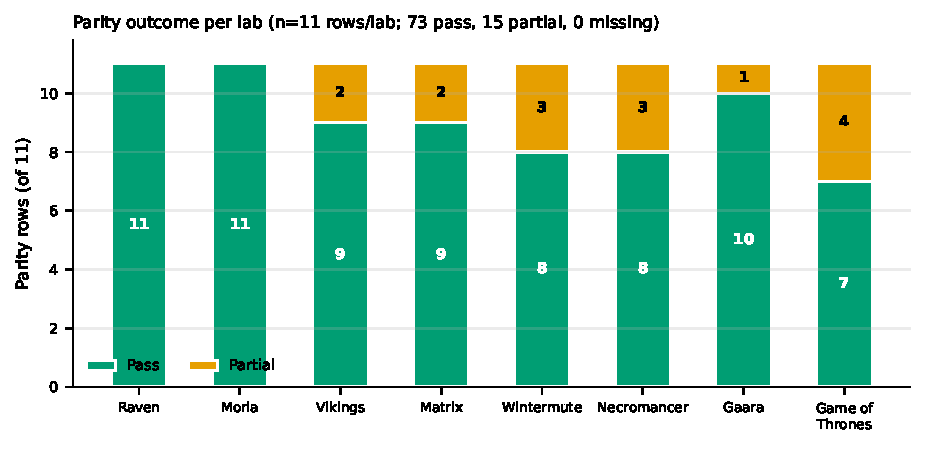
\includegraphics[width=\textwidth]{figures/fig04_parity_stacked.pdf}
\caption{Pass/partial rows per lab ($n=11$ rows per lab). No row in any
lab is missing: every partial is a present function with a named
substitution, not an absence.}
\label{fig:parity}
\end{figure*}

The anatomy of the 15 partial rows is concentrated, not diffuse
(Table~\ref{tab:areas}, Figures~\ref{fig:heatmap} and
\ref{fig:radar}). Four areas pass on every lab---unpublished loopback
services, users, sudoers, and the application URL---which is to say
the security topology and the identity surface are the most
reproducible parts of these guests. Virtual hosts, web paths,
databases, cron, and mail each fail strict pass once. The two
systematic weaknesses are \textbf{package versions (partial in 6 of 8
labs; strict pass rate 25\%)} and \textbf{listening ports (4 of 8;
50\%)}, and their causes are classifiable (Table~\ref{tab:causes}):

\begin{itemize}
\item \emph{Archive-revision drift} (Gaara, Game of Thrones, Wintermute,
and the archive component in Vikings): the EOL archive serves a newer
security revision than the guest carried. The function is identical;
the string is not, and the rubric scores strings.
\item \emph{Unreproducible guest substrate} (Matrix's Slackware packages on a Debian base; Necromancer's OpenBSD base, \texttt{httpd},
and periodic scripts on Debian~11): no Linux container base exists, so
the row is partial by construction.
\item \emph{Guest-runtime collapse} (Vikings' systemd-resolved and
containerd listeners; Game of Thrones' guest Docker engine and its
nine images; Wintermute's un-recreated second guest services):
listeners or engines that existed only as guest-runtime state are
replaced by named stand-ins (e.g., nginx for the guest's port-10000
service, MariaDB for its MySQL image, Dovecot for its mail image) or
recorded unbound until use (FTP passive range).
\item \emph{Single-string drift} (Wintermute mail: Postfix
\texttt{3.1.15-0+deb9u1} for \texttt{3.1.8-0+deb9u1}): one defining
string differs while the service is otherwise the guest's.
\end{itemize}

\begin{table}[tbp]
\caption{Strict pass by rubric area (8 labs). Users, sudoers, loopback
containment, and the application URL are universally reproduced;
package versions and listening ports are not.}
\label{tab:areas}
\centering\footnotesize
\begin{tabularx}{\columnwidth}{Xrr}
\toprule
Area & Pass & Partial\\
\midrule
Listening ports & 4 & 4\\
Loopback unpublished & 8 & 0\\
Package versions & 2 & 6\\
Users & 8 & 0\\
Sudoers & 8 & 0\\
Virtual hosts & 7 & 1\\
Web paths & 7 & 1\\
Databases & 7 & 1\\
Cron & 7 & 1\\
Mail & 7 & 1\\
Application URL & 8 & 0\\
\bottomrule
\end{tabularx}
\end{table}

\begin{figure*}[tbp]
\centering
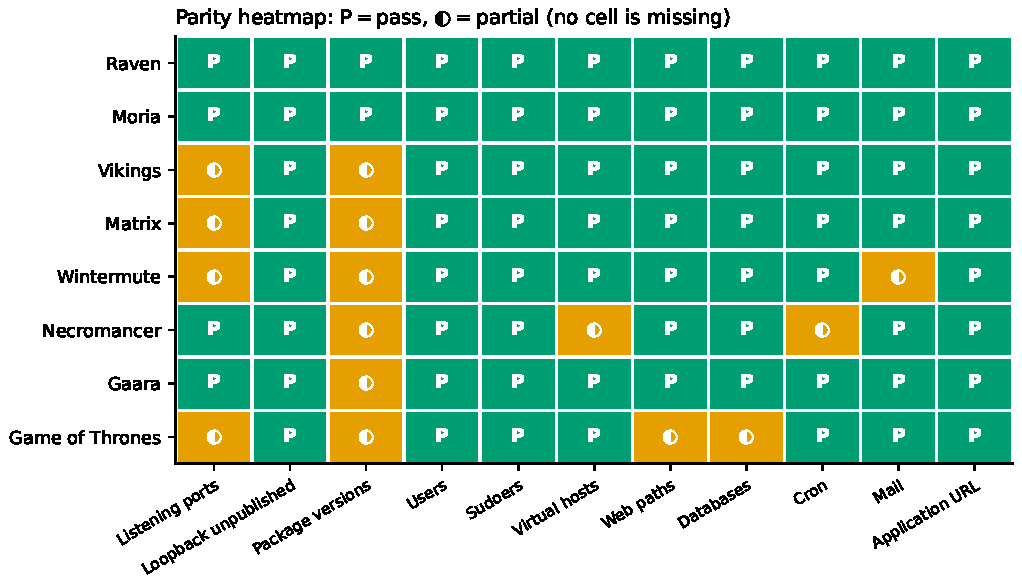
\includegraphics[width=0.92\textwidth]{figures/fig05_heatmap.pdf}
\caption{Parity heatmap (labs $\times$ areas). Partials cluster in the
package-version column (six labs) and the listening-port column (four
labs); identity, privilege, containment, and URL columns are uniformly
pass.}
\label{fig:heatmap}
\end{figure*}

\begin{figure}[tbp]
\centering
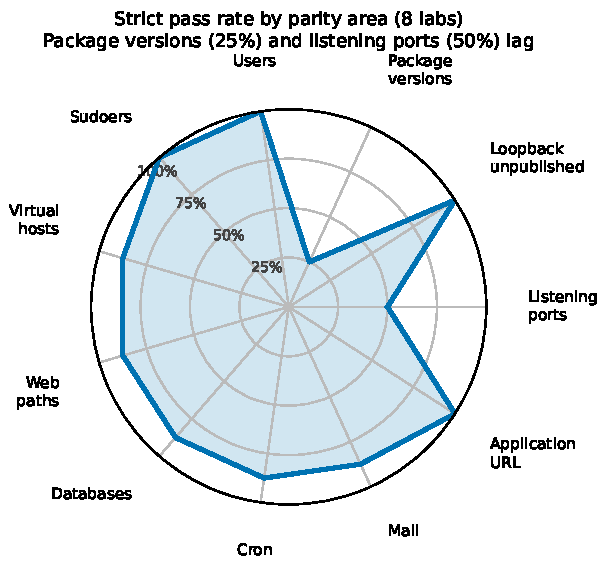
\includegraphics[width=\columnwidth]{figures/fig08_radar_areas.pdf}
\caption{Spider (radar) view of strict pass rate by area. The two
indentations---package versions (25\%) and listening ports (50\%)---are
the corpus's fidelity frontier; all other areas sit at 87.5--100\%.}
\label{fig:radar}
\end{figure}

\begin{table*}[tbp]
\caption{Root-cause classification of all 15 partial rows (primary
corpus). A row may carry one primary cause; counts sum to 15.}
\label{tab:causes}
\centering\footnotesize
\begin{tabularx}{\textwidth}{lclX}
\toprule
Cause & Rows & Labs & Mechanism\\
\midrule
Archive-revision drift & 5 & Gaara, Vikings, Wintermute (pkg), GoT, Wintermute (mail) & Archive serves newer EOL security revision than guest string\\
Unreproducible substrate & 3 & Matrix (pkg), Necromancer (pkg, vhosts) & Slackware/OpenBSD cannot be the Linux container base\\
Guest-runtime collapse & 4 & Vikings (ports), GoT (ports, web, DB) & Guest-runtime state replaced by stand-ins or uncopied trees\\
Live-evidence unavailable & 2 & Matrix (ports), Wintermute (ports) & Guest never booted; listener row rests on startup/config files\\
Substitution disclosed & 1 & Necromancer (cron) & Added job present; BSD periodic programs absent\\
\bottomrule
\end{tabularx}
\end{table*}

\subsubsection{RQ2---Configured memory and its relation to fidelity}

Configured replica caps total \textbf{5,248~MB against 8,168~MB} of
guest RAM---2,920~MB (35.7\%) less configuration for the same published
port surface (Figure~\ref{fig:memory}). Per lab, caps are at or below
the guest allocation by construction (the build skill forbids exceeding
it): Raven is equal (512/512~MB, because Jessie-era services were
sized to the guest), Moria, Vikings, Wintermute, and Gaara halve the
allocation, Matrix and Necromancer retain 75\%, and Game of Thrones
retains 93.1\% (1,408 of 1,512~MB, the sum of nine container caps).
Guest RAM and cap are strongly rank-associated (Spearman
$\rho=0.87$, $n=8$; Figure~\ref{fig:scatter-ram}), which is expected
because the cap rule is defined relative to the guest; we report it as
a design check, not a discovery. The substantive question---whether
larger savings cost fidelity---shows no evident association in this
corpus (saving vs.\ pass rows: $\rho=0.14$, $n=8$, exploratory;
Figure~\ref{fig:scatter-explore}b). Fidelity instead tracks
topological complexity: replicas with more containers pass fewer rows
($\rho=-0.72$, $n=8$, exploratory; Figure~\ref{fig:scatter-explore}a),
driven by Game of Thrones (9 containers, 7 passes) and Wintermute
(2 guests, 8 passes) against five single-container labs at 8--11
passes. With eight heterogeneous cases both correlations are
hypothesis-generating only. And the boundary of the claim matters:
caps bound what the engine \emph{may} allocate. No resident memory,
startup time, or throughput was measured, so no operational saving is
claimed---only that the laboratory's published surface is configured
to run inside a smaller envelope, consistent with the direction (not
the magnitude) of container/VM comparisons in the literature
\citep{felter2015, nakata2021}.

\begin{figure*}[tbp]
\centering
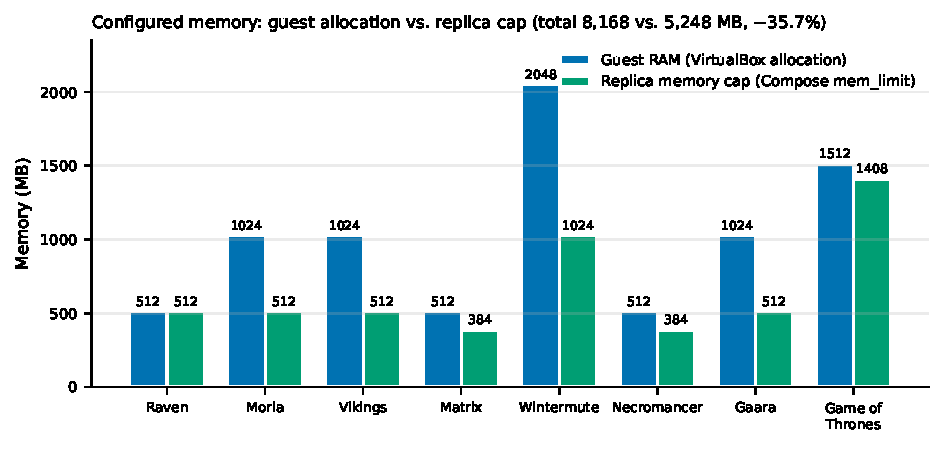
\includegraphics[width=\textwidth]{figures/fig03_memory_grouped.pdf}
\caption{Configured memory by lab: VirtualBox guest allocation vs.\
Compose memory cap. Wintermute aggregates two guests (1,024~MB each)
and two containers (512~MB each); Game of Thrones aggregates nine
containers (256 $+$ $6\times128$ $+$ $2\times192$~MB).}
\label{fig:memory}
\end{figure*}

\begin{figure}[tbp]
\centering
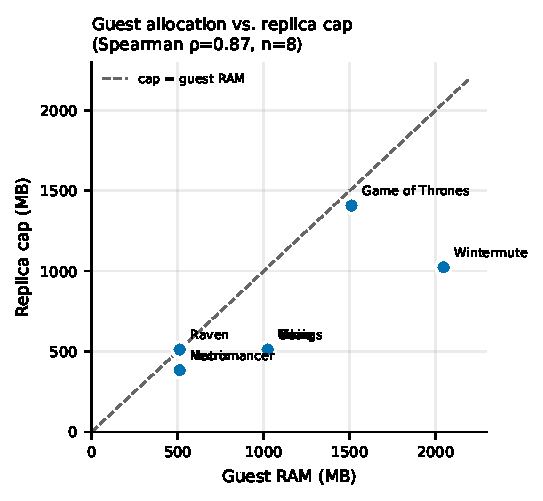
\includegraphics[width=\columnwidth]{figures/fig06_scatter_ram_cap.pdf}
\caption{Guest allocation vs.\ replica cap with the identity line.
Every lab sits on or below the line by rule; rank association
($\rho=0.87$) reflects the capping rule, not an empirical law.}
\label{fig:scatter-ram}
\end{figure}

\begin{figure*}[tbp]
\centering
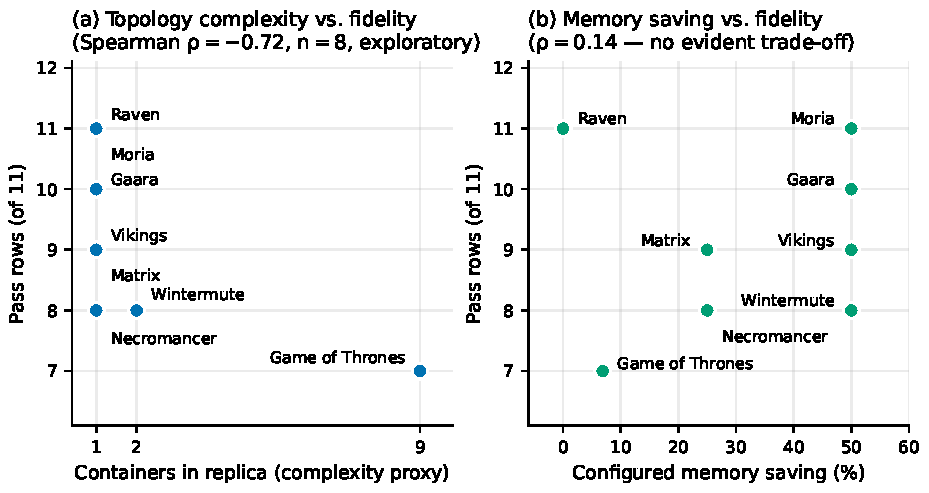
\includegraphics[width=\textwidth]{figures/fig10_scatter_exploratory.pdf}
\caption{Exploratory associations ($n=8$; hypothesis-generating only).
(a)~Fidelity falls as replica container count rises.
(b)~Fidelity shows no evident association with configured memory
saving. Together they suggest complexity, not frugality, is the
fidelity risk in this corpus.}
\label{fig:scatter-explore}
\end{figure*}

\subsubsection{RQ3---What codifying the rules changed (Raven)}

Raven is the one lab scored twice on the same eleven rows: before the
conversion rules were written into the skills (Round~1) and after the
procedure was applied and the newly discovered traps were written back
(Round~2). The replica went from \textbf{5 pass / 6 partial / 0 missing
(45.5\% strict pass) to 11 pass / 0 partial (100\%)}
(Figure~\ref{fig:raven}). Table~\ref{tab:raven} names the six fixes.
Each maps to a skill sentence that now exists independently of Raven:
rebuild from the guest codename and pin the inventoried revisions;
install the inventoried database engine on a fresh volume; install the
package that owns a missing listener (\texttt{nfs-common} /
\texttt{rpc.statd}); keep the distribution's PHP cron snippet;
supervise Sendmail in the foreground and score its sockets after the
startup minute; and preserve the stored application URL by mapping the
hostname to the published address. Round~1 is instructive precisely
because the container \emph{worked}: it answered HTTP with Debian~9
packages and MariaDB~10.1 standing in for Debian~8 and MySQL~5.5.
Under a ``page loads'' criterion the conversion was finished; under
parity, six rows were partial. The structural gaps did not move:
archive/snapshot apt with \texttt{trusted=yes} on the archived lines,
the WSL host kernel (6.18.x) in place of the guest's
\texttt{3.16.0-6-amd64}, and supervisord in place of sysv init remain
in Raven's gap register in Round~2. That separation---rows improvable
to pass, gaps permanently disclosed---is the rubric working as
designed.

We state the inferential limit plainly. This is one case, scored by the
project, with the rebuild and the rule-writing entangled: Round~2
differs from Round~1 both because the rules existed and because the
replica was rebuilt under them. Rows within the case are not
independent observations, and no statistical test is applied. The
claim is therefore mechanistic, not causal-population: the six
Round~1 failure modes are each addressed by a named rule, and the
rescored artifact passes the rows those rules govern. Whether a
\emph{different} agent, given only the skills, reaches Round~2 on a
\emph{new} appliance without assistance is the decisive test and has
not been run (Section~\ref{sec:discussion}).

\begin{figure*}[tbp]
\centering
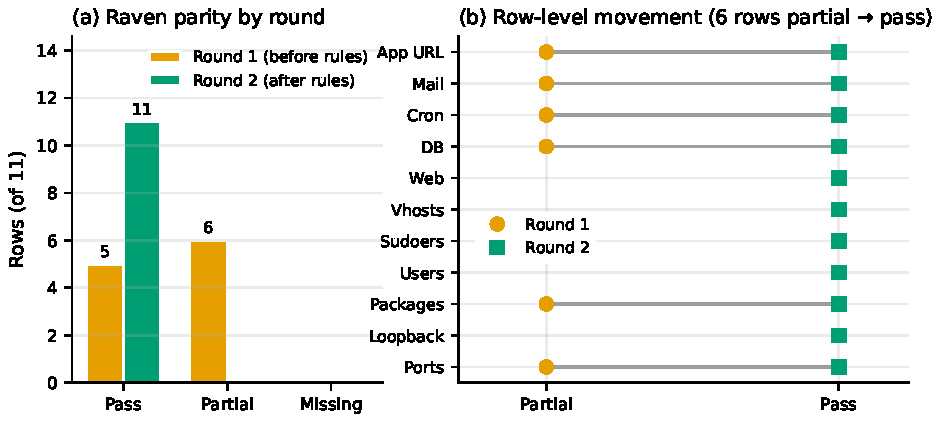
\includegraphics[width=\textwidth]{figures/fig07_raven_longitudinal.pdf}
\caption{Raven longitudinal comparison ($n=11$ rows). (a)~Row counts by
round. (b)~Row-level dumbbell: six rows move partial$\rightarrow$pass;
five were already pass; none is missing in either round. The gap
register (archive apt, shared kernel, supervisor) is unchanged and is
not part of the 11 rows.}
\label{fig:raven}
\end{figure*}

\begin{table*}[tbp]
\caption{The six Raven rows that changed between rounds, the codified
fix, and the governing skill rule. Rows already passing (loopback,
users, sudoers, vhosts, web paths) required no fix.}
\label{tab:raven}
\centering\footnotesize
\begin{tabularx}{\textwidth}{lXX}
\toprule
Row (Round 1 $\rightarrow$ 2) & Fix applied & Rule now codified\\
\midrule
Ports: partial $\rightarrow$ pass & Install \texttt{nfs-common}; run \texttt{rpcbind} + foreground \texttt{rpc.statd} & Score every inventoried listener from \texttt{ss}; a missing daemon is a build defect, not a note\\
Packages: partial $\rightarrow$ pass & Rebuild \texttt{FROM debian:jessie}; pin guest revisions via dated snapshots & Do not call the row a pass until \texttt{dpkg-query} matches inventory strings\\
Databases: partial $\rightarrow$ pass & Install \texttt{mysql-server} 5.5.60 on a fresh volume (MariaDB removed) & Install the inventoried engine; never mount one engine's data dir into the other\\
Cron: partial $\rightarrow$ pass & Keep the distro php5 \texttt{cron.d} snippet & A package-owned snippet absent from the replica is a partial row\\
Mail: partial $\rightarrow$ pass & Pin Sendmail 8.14.4; supervise \texttt{sendmail -bD}; score after $\approx$60 s & Score mail from sockets after the startup window, never from early supervisor status\\
App.\ URL: partial $\rightarrow$ pass & Keep \texttt{http://raven.local/wordpress/}; map the name to 10.88.10.10 & Map the hostname to the published address; do not rewrite the stored URL\\
\bottomrule
\end{tabularx}
\end{table*}

\subsubsection{RQ4---Where the rules reside}
\label{sec:rq4}

Experiment~A (cross-lab, 13~October~2026) searched the 23 coded rule
sentences in the three skill files and, separately, in each primary
lab's finished files (Table~\ref{tab:lookup},
Figure~\ref{fig:lookup}). The skills contain all 23 sentences
(23/23). The eight lab corpora contain \textbf{7 hits in 184
opportunities (3.8\%)}: seven labs contain exactly one sentence---the
\texttt{Acquire::Check-Valid-Until "false"} assignment that necessarily
survives into a Dockerfile or sources list---and Moria contains none,
because its CentOS vault repair never writes the Debian assignment.
In other words, 22 of the 23 decision rules (when \texttt{trusted=yes}
is legal, which ports stay unpublished, why MariaDB-for-MySQL remains
partial, why the kernel is never a pass, how long to wait before
scoring mail) are textually absent from the artifacts a skills-less
agent would inherit. Experiment~B (per-lab files, seven labs) replicates
the coverage result on independently assembled corpora: skills 23/23 in
every lab's run; replica files 1/23 in every lab, again the
\texttt{Check-Valid-Until} line.

\begin{table}[tbp]
\caption{Experiment~A: exact-string lookup of 23 rule sentences
(13 Oct 2026, five repetitions, median of five). Times are script
file-read times. Experiment~B per-lab medians (skills vs.\ replica
files) were: Gaara 1.900/3.461~ms, Game of Thrones 1.874/4.284~ms,
Matrix 0.593/0.562~ms, Necromancer 1.724/4.127~ms, Vikings
0.618/0.635~ms, Wintermute 0.758/1.039~ms (MrRobot, sensitivity:
2.129/4.050~ms); coverage was 23/23 vs.\ 1/23 in every run.}
\label{tab:lookup}
\centering\footnotesize
\begin{tabularx}{\columnwidth}{Xrrr}
\toprule
Corpus & Files & Hits & Median (ms)\\
\midrule
Three skills & 3 & 23/23 & 2.539\\
Raven files & 8 & 1/23 & 5.076\\
Moria files & 5 & 0/23 & 3.123\\
Vikings files & 6 & 1/23 & 3.532\\
Matrix files & 6 & 1/23 & 3.589\\
Wintermute files & 9 & 1/23 & 4.862\\
Necromancer files & 9 & 1/23 & 4.835\\
Gaara files & 7 & 1/23 & 3.641\\
Game of Thrones files & 9 & 1/23 & 4.553\\
\bottomrule
\end{tabularx}
\end{table}

\begin{figure*}[tbp]
\centering
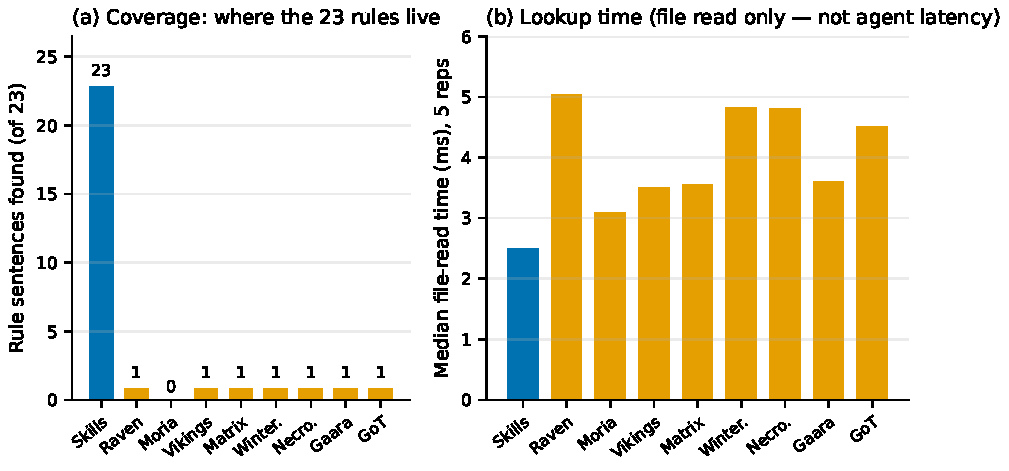
\includegraphics[width=\textwidth]{figures/fig09_lookup.pdf}
\caption{Experiment~A. (a)~Coverage is the result: the rules live in
the skills (23/23) and not in finished lab files (0--1/23).
(b)~Median file-read times differ by milliseconds and carry no agent
meaning; they are shown to preclude, not support, a latency reading.}
\label{fig:lookup}
\end{figure*}

The timing columns require the paper's most explicit non-claim. All
corpora are read in single-digit milliseconds (skills median 2.539~ms;
lab medians 3.123--5.076~ms in Experiment~A; 0.562--4.284~ms across
Experiment~B), repetition~1 is the cold read (e.g., 8.842~ms for the
skills corpus in Experiment~A), and the ordering between corpora is
not even consistent across experiments. These are measurements of a
script that already knows the sentence it is looking for. They are not
LM task times, they do not show that an agent with the skills is
faster, and we draw no speed conclusion from them. The qualitative
speed-adjacent observation the sessions do support is avoided
iteration: before codification, the Raven conversion spent rebuilds on
the wrong suite and engine and probed Sendmail inside its startup
minute; the codified rules remove those specific iterations from the
next conversion by stating the base, engine, flag, and wait in
advance. Testing whether that removal materialises as agent time saved
requires timing a second agent, which was not done.


\section{Discussion}
\label{sec:discussion}

\subsection{What the results mean}

Three findings survive the paper's own caveats. First, \emph{container
replicas of owned appliances can be made configuration-faithful, but
fidelity is a scored property, not a by-product of a working build.}
Every replica in the corpus answered on its published address, yet the
strict pass rate is 83.0\%, not 100\%, and the shortfall is
concentrated exactly where casual verification does not look: package
revision strings and the full listener set. A ``does it respond?''
acceptance test---the analogue of accepting an agent's plausible
narrative \citep{jimenez2024}---would have reported eight successes
and hidden fifteen substitutions.

Second, \emph{the fidelity frontier is archival, not structural.}
Identity, privilege, containment, and application state transferred
perfectly (32 of 32 rows across users, sudoers, loopback, and URL);
what resisted transfer is the past itself. EOL archives serve newer
revisions than guests carried, non-Linux guests have no container
base, and guest-runtime state (a Docker engine inside the guest,
systemd-resolved's ephemeral listener) has no file to copy. This
reframes VM-to-container conversion as a problem in \emph{software
archaeology under trust constraints}: the snapshot-pinning and
vault-mirror mechanisms that recovered the only two package-row passes
(Raven, Moria) are the same mechanisms \citet{caneill2017} and
\citet{lamb2022} motivate for historical and reproducible builds, and
the rubric's refusal to call a newer revision a pass is what makes
their use auditable rather than cosmetic.

Third, \emph{the durable contribution of an agent session is the
procedure it leaves behind.} Raven's six fixed rows were not fixed by
a better single build; they were fixed by converting session
discoveries into preconditioned rules with stop conditions, after
which the rescore moved. RQ4 sharpens the point negatively: the
finished files retain one of 23 rules, so an agent (or a human)
starting from the artifacts alone inherits the answers without the
criteria that distinguish a pass from a confident partial. That is a
general hazard for LM-assisted systems work as its outputs accumulate:
\emph{artifacts under-specify the evaluations that legitimised them},
and evaluations therefore need to be published as first-class,
re-runnable artifacts alongside the builds they score---here, the
skills, the inventories, and the parity reports.

\subsection{Security implications}

The parity discipline is also a containment discipline. The
loopback-unpublished row passing on all eight labs (plus MrRobot)
means no replica silently widened its guest's attack surface:
databases, mail submission, Redis, SNMP, and admin listeners that the
guests kept private stayed private, while published surfaces kept the
guest's own port numbers, preserving the enumeration lesson the lab
exists to teach \citep{thompson2018, yamin2020}. Conversely, the rubric
treats widening as the severest outcome (a missing row), which inverts
the usual convenience gradient under which exposing a database
``temporarily, for debugging'' is costless. The EOL trust rules carry
the second security implication: \texttt{trusted=yes} and disabled
validity checking are necessary to install EOL guests at all, and are
therefore precisely the settings that must be line-scoped,
failure-triggered, and permanently registered as gaps, lest a repair
for a 2015 suite become a standing policy for current mirrors. Finally,
nothing in the conversion requires attacking the guest: administration
is recovered offline on a clone, inventory stops at version recording,
and reports are secret-free by construction, which keeps the workflow
inside the authorisation boundary of owned appliances. The student
surface strengthens the same properties---current base, no root SSH,
learner-chosen credentials---so the teaching artifact does not
re-distribute the historical vulnerable system it describes. None of
this makes a replica \emph{safe} in the container-security sense:
replicas intentionally run old, vulnerable services and inherit the
shared-kernel exposure \citet{sultan2019} catalogue; they belong on
isolated laboratory networks, which the dedicated-address publication
model is designed to enforce.

\subsection{Threats to validity}

\paragraph{Construct validity.}
Parity is configuration equality against an inventory, not behavioural
equivalence: we did not fuzz services, replay workloads, or verify
that an exercise's full solution path survives conversion, and a
pass row for ``web paths'' evidences presence and HTTP status, not
byte-identical application behaviour in all cases (Game of Thrones'
uncopied web trees are scored partial for this reason). Memory results
are configured caps, not residency, latency, or throughput
measurements. The lookup study measures textual residence of rules,
not agent comprehension or task success.

\paragraph{Internal validity.}
Row scoring was performed by the project that built the replicas,
against its own rubric, without independent re-scoring; the Raven
before/after comparison entangles rule codification with the rebuild
itself and with scorer learning. Five of eight inventories rest on
configuration evidence from unbooted guests, so their listener rows
could err in either direction (a configured service that would not
have started; a started service with no surviving configuration).
The exploratory correlations use eight heterogeneous cases and are
reported without inferential claims.

\paragraph{External validity.}
The corpus is the project's owned appliances: small, old, Linux/BSD,
web-and-SSH-centric boot-to-root systems on one Windows/WSL2 +
VirtualBox host. Results should not be extrapolated to Windows guests,
current distributions, cloud ranges, multi-host enterprise scenarios
\citep{chouliaras2023}, or conversions performed by other agents or
humans. The one population the results do speak to---educators and
range operators holding similar legacy appliances---is the population
the skills address.

\paragraph{Reliability.}
The audit script re-derives headline counts from the primary files and
is retained with the paper materials, as are the sentence set, the
per-lab experiment files, and the figure-generation script from the
same dataset table that the audit validated. Independent replication
requires the owned appliances (not redistributable) but not the
sessions: skills, inventories, Dockerfiles, Compose files, and parity
reports suffice to re-score every row except those requiring a booted
guest, whose provenance is marked.

\subsection{Limitations and future work}

The decisive unrun experiment is a \emph{second-agent study}: give an
LM agent that has not seen the sessions a new owned appliance, with
and without the skills, and measure parity outcome and task time under
the same rubric. Until that is run, RQ3--RQ4 support a residence and
mechanism claim, not an efficacy or speedup claim. Three engineering
evaluations are similarly open: measured (rather than configured)
memory, startup, and throughput of replicas against their guests, in
the manner of \citet{felter2015} and \citet{nakata2021}; behavioural
exercise-level validation (can each lab's documented learning path be
completed against the replica, and does automated assessment agree
with the VM's, as in Labtainers-style grading \citep{thompson2018});
and independent re-scoring of the 88 rows to estimate rubric
reliability. On the method side, the rubric should grow rows the
current corpus did not force---kernel-adjacent behaviour, filesystem
state beyond web trees, and timing behaviour---and the scenario-design
skill's outputs should be evaluated pedagogically (learning outcomes,
not only topology well-formedness) before classroom claims are made.
The corrected README sentence (audit item~1) should be fixed upstream
so the narrative record again matches the scored artifacts.

\section{Conclusion}
\label{sec:conclusion}

An owned virtual appliance and a container that answers on the same
ports are not automatically the same laboratory. This paper supplied
the missing middle: a six-skill conversion procedure with stop
conditions, an eleven-row parity rubric that scores configuration
equality from live evidence, and a gap register that keeps archive
trust, the shared host kernel, and supervisor-for-init permanently
visible instead of letting them be scored away. Across eight replicas
(88 rows), the procedure yields 73 passes, 15 named partials, and no
missing rows, inside configured memory envelopes totalling 35.7\% less
than the guests' RAM allocations; package-revision archaeology and
listener completeness, not identity, privilege, containment, or
application state, are where fidelity is won and lost. Codifying the
procedure moved the one longitudinally scored replica from five to
eleven passing rows, and the rules that did so demonstrably live in
the skill documents rather than in the finished builds (23/23 vs.\
7/184 lab-file hits). The claims are deliberately bounded---no
measured residency, no second-agent timing, no kernel equivalence---
because the paper's central argument is that bounded, checkable
claims are the product. For educators and range operators holding
legacy appliances, the artifact set (skills, redacted inventories,
pinned builds, parity reports, and teaching modules) offers a way to
retire the hypervisor seat without retiring the host the lesson was
about---and to prove, row by row, what survived the move.

\section*{Acknowledgements}
The authors thank the maintainers of the community appliances and of
the Debian, Ubuntu, and CentOS archives and snapshot services on which
the EOL repairs depend. Appliance names are used to identify the owned
laboratory systems studied.

\section*{CRediT authorship contribution statement}
\textbf{ZeroCrowd-Labs Project Team:} Conceptualisation, Methodology,
Software, Validation, Formal analysis, Investigation, Data curation,
Writing---original draft, Writing---review and editing, Visualisation.
Individual contributor names and roles to be completed on submission.

\section*{Declaration of competing interest}
The authors declare that they have no known competing financial
interests or personal relationships that could have appeared to
influence the work reported in this paper.

\section*{Data availability}
The conversion skills, redacted guest inventories, Dockerfiles,
Compose files, parity reports, lookup sentence set, validation script,
and figure-generation code are available in the ZeroCrowd-Labs
repository accompanying this manuscript. Guest disk images, appliance
archives, credentials, and shadow material are not shared: they are
neither necessary to re-score the reported rows nor redistributable.


\begin{thebibliography}{25}
\footnotesize

\bibitem[Bernstein(2014)]{bernstein2014}
Bernstein, D. (2014). Containers and cloud: From LXC to Docker to
Kubernetes. \textit{IEEE Cloud Computing}, \textit{1}(3), 81--84.
\url{https://doi.org/10.1109/MCC.2014.51}

\bibitem[Boettiger(2015)]{boettiger2015}
Boettiger, C. (2015). An introduction to Docker for reproducible
research. \textit{ACM SIGOPS Operating Systems Review}, \textit{49}(1),
71--79. \url{https://doi.org/10.1145/2723872.2723882}

\bibitem[Caneill et~al.(2017)]{caneill2017}
Caneill, M., Germ\'an, D. M., \& Zacchiroli, S. (2017). The Debsources
dataset: Two decades of free and open source software.
\textit{Empirical Software Engineering}, \textit{22}(3), 1405--1437.
\url{https://doi.org/10.1007/s10664-016-9461-5}

\bibitem[Chouliaras et~al.(2023)]{chouliaras2023}
Chouliaras, N., Kantzavelou, I., Maglaras, L., Pantziou, G., \& Ferrag,
M. A. (2023). A novel autonomous container-based platform for
cybersecurity training and research. \textit{PeerJ Computer Science},
\textit{9}, Article e1574. \url{https://doi.org/10.7717/peerj-cs.1574}

\bibitem[Du et~al.(2007)]{du2007}
Du, W., Teng, Z., \& Wang, R. (2007). SEED: A suite of instructional
laboratories for computer security education. In \textit{Proceedings of
the 38th ACM Technical Symposium on Computer Science Education}
(pp.~486--490). Association for Computing Machinery.
\url{https://doi.org/10.1145/1227504.1227474}

\bibitem[Felter et~al.(2015)]{felter2015}
Felter, W., Ferreira, A., Rajamony, R., \& Rubio, J. (2015). An updated
performance comparison of virtual machines and Linux containers. In
\textit{Proceedings of the 2015 IEEE International Symposium on
Performance Analysis of Systems and Software (ISPASS)} (pp.~171--172).
IEEE. \url{https://doi.org/10.1109/ISPASS.2015.7095802}

\bibitem[Guerriero et~al.(2019)]{guerriero2019}
Guerriero, M., Garriga, M., Tamburri, D. A., \& Palomba, F. (2019).
Adoption, support, and challenges of infrastructure-as-code: Insights
from industry. In \textit{Proceedings of the 2019 IEEE International
Conference on Software Maintenance and Evolution (ICSME)}
(pp.~580--589). IEEE. \url{https://doi.org/10.1109/ICSME.2019.00092}

\bibitem[Haynes et~al.(2009)]{haynes2009}
Haynes, A. B., Weiser, T. G., Berry, W. R., Lipsitz, S. R., Breizat,
A.-H. S., Dellinger, E. P., Herbosa, T., Joseph, S., Kibatala, P. L.,
Lapitan, M. C. M., Merry, A. F., Moorthy, K., Reznick, R. K., Taylor,
B., \& Gawande, A. A. (2009). A surgical safety checklist to reduce
morbidity and mortality in a global population. \textit{The New
England Journal of Medicine}, \textit{360}(5), 491--499.
\url{https://doi.org/10.1056/NEJMsa0810119}

\bibitem[Hummer et~al.(2013)]{hummer2013}
Hummer, W., Rosenberg, F., Oliveira, F., \& Eilam, T. (2013). Testing
idempotence for infrastructure as code. In D. Eyers \& K. Schwan
(Eds.), \textit{Middleware 2013} (Lecture Notes in Computer Science,
Vol.~8275, pp.~368--388). Springer.
\url{https://doi.org/10.1007/978-3-642-45065-5\_19}

\bibitem[Jimenez et~al.(2024)]{jimenez2024}
Jimenez, C. E., Yang, J., Wettig, A., Yao, S., Pei, K., Press, O., \&
Narasimhan, K. (2024). SWE-bench: Can language models resolve real-world
GitHub issues? In \textit{Proceedings of the Twelfth International
Conference on Learning Representations}.
\url{https://proceedings.iclr.cc/paper\_files/paper/2024/hash/edac78c3e300629acfe6cbe9ca88fb84-Abstract-Conference.html}

\bibitem[Kitchenham et~al.(2002)]{kitchenham2002}
Kitchenham, B. A., Pfleeger, S. L., Pickard, L. M., Jones, P. W.,
Hoaglin, D. C., El Emam, K., \& Rosenberg, J. (2002). Preliminary
guidelines for empirical research in software engineering.
\textit{IEEE Transactions on Software Engineering}, \textit{28}(8),
721--734. \url{https://doi.org/10.1109/TSE.2002.1027796}

\bibitem[Lamb \& Zacchiroli(2022)]{lamb2022}
Lamb, C., \& Zacchiroli, S. (2022). Reproducible builds: Increasing the
integrity of software supply chains. \textit{IEEE Software},
\textit{39}(2), 62--70. \url{https://doi.org/10.1109/MS.2021.3073045}

\bibitem[Merkel(2014)]{merkel2014}
Merkel, D. (2014). Docker: Lightweight Linux containers for consistent
development and deployment. \textit{Linux Journal}, \textit{2014}(239),
Article~2.

\bibitem[Naik(2016)]{naik2016}
Naik, N. (2016). Migrating from virtualization to Dockerization in the
cloud: Simulation and evaluation of distributed systems. In
\textit{Proceedings of the 2016 IEEE 10th International Symposium on
the Maintenance and Evolution of Service-Oriented and Cloud-Based
Environments (MESOCA)} (pp.~1--8). IEEE.
\url{https://doi.org/10.1109/MESOCA.2016.9}

\bibitem[Nakata \& Otsuka(2021)]{nakata2021}
Nakata, R., \& Otsuka, A. (2021). CyExec*: A high-performance
container-based cyber range with scenario randomization.
\textit{IEEE Access}, \textit{9}, 109095--109114.
\url{https://doi.org/10.1109/ACCESS.2021.3101245}

\bibitem[N\"ust et~al.(2020)]{nust2020}
N\"ust, D., Sochat, V., Marwick, B., Eglen, S. J., Head, T., Hirst, T.,
\& Evans, B. D. (2020). Ten simple rules for writing Dockerfiles for
reproducible data science. \textit{PLOS Computational Biology},
\textit{16}(11), Article e1008316.
\url{https://doi.org/10.1371/journal.pcbi.1008316}

\bibitem[Runeson \& H\"ost(2009)]{runeson2009}
Runeson, P., \& H\"ost, M. (2009). Guidelines for conducting and
reporting case study research in software engineering.
\textit{Empirical Software Engineering}, \textit{14}, 131--164.
\url{https://doi.org/10.1007/s10664-008-9102-8}

\bibitem[Schreuders et~al.(2017)]{schreuders2017}
Schreuders, Z. C., Shaw, T., Shan-A-Khuda, M., Ravichandran, G.,
Keighley, J., \& Ordean, M. (2017). Security scenario generator
(SecGen): A framework for generating randomly vulnerable rich-scenario
VMs for learning computer security and hosting CTF events. In
\textit{Proceedings of the 2017 USENIX Advances in Security Education
Workshop (ASE~'17)}. USENIX Association.

\bibitem[Shambaugh et~al.(2016)]{shambaugh2016}
Shambaugh, R., Weiss, A., \& Guha, A. (2016). Rehearsal: A configuration
verification tool for Puppet. In \textit{Proceedings of the 37th ACM
SIGPLAN Conference on Programming Language Design and Implementation}
(pp.~416--430). Association for Computing Machinery.
\url{https://doi.org/10.1145/2908080.2908083}

\bibitem[Sultan et~al.(2019)]{sultan2019}
Sultan, S., Ahmad, I., \& Dimitriou, T. (2019). Container security:
Issues, challenges, and the road ahead. \textit{IEEE Access},
\textit{7}, 52976--52996. \url{https://doi.org/10.1109/ACCESS.2019.2911732}

\bibitem[Thompson \& Irvine(2018)]{thompson2018}
Thompson, M. F., \& Irvine, C. E. (2018). Individualizing cybersecurity
lab exercises with Labtainers. \textit{IEEE Security \& Privacy},
\textit{16}(2), 91--95. \url{https://doi.org/10.1109/MSP.2018.1870862}

\bibitem[Ukwandu et~al.(2020)]{ukwandu2020}
Ukwandu, E., Farah, M. A. B., Hindy, H., Brosset, D., Kavallieros, D.,
Atkinson, R., Tachtatzis, C., Bur\'es, M., Andonovic, I., \& Bellekens,
X. (2020). A review of cyber-ranges and test-beds: Current and future
trends. \textit{Sensors}, \textit{20}(24), Article 7148.
\url{https://doi.org/10.3390/s20247148}

\bibitem[Wohlin et~al.(2012)]{wohlin2012}
Wohlin, C., Runeson, P., H\"ost, M., Ohlsson, M. C., Regnell, B., \&
Wessl\'en, A. (2012). \textit{Experimentation in software engineering}.
Springer.

\bibitem[Yamin et~al.(2020)]{yamin2020}
Yamin, M. M., Katt, B., \& Gkioulos, V. (2020). Cyber ranges and
security testbeds: Scenarios, functions, tools and architecture.
\textit{Computers \& Security}, \textit{88}, Article 101636.
\url{https://doi.org/10.1016/j.cose.2019.101636}

\bibitem[Yao et~al.(2023)]{yao2023}
Yao, S., Zhao, J., Yu, D., Du, N., Shafran, I., Narasimhan, K. R., \&
Cao, Y. (2023). ReAct: Synergizing reasoning and acting in language
models. In \textit{Proceedings of the Eleventh International
Conference on Learning Representations}.
\url{https://iclr.cc/virtual/2023/poster/11003}

\end{thebibliography}

\end{document}
